\documentclass[xcolor=svgnames,dvipsnames,table, hyperref=pdftex, mathserif, presentation]{beamer}
\usepackage{amsmath,amssymb,amsfonts,amsthm}
\usepackage{ctex}
\setCJKsansfont{KaiTi}% 文泉驿的黑体
\usepackage{graphics}
\usepackage{graphicx}
\usepackage{xcolor}
\usepackage{wasysym}
\usepackage{bbm}
\usepackage{url}
\usepackage{beamerleanprogress}
\usepackage{tikz-dependency}
\usepackage{tikz-qtree}
\usepackage{hhline}
\usepackage{fancyvrb}
\usepackage{mathrsfs}
\usepackage{alltt}
% for uml charts
\usepackage{tikz}
\usetikzlibrary{calc,arrows.meta, graphs, trees, shapes, positioning, automata,
shapes.geometric, shapes.multipart, er, patterns, decorations.markings, intersections, decorations.text}
\usepackage{tikz-uml}

\usetheme{CambridgeUS}
%\usetheme{Pittsburgh}
\usecolortheme{orchid} % seahorse  orchid rose
\setbeamertemplate{blocks}[rounded][shadow=true]
\AtBeginSection[]{%
  \begin{frame}<beamer>
    \frametitle{Outline}
      \tableofcontents[current] 
    \end{frame}
  \addtocounter{framenumber}{-1}% If you don't want them to affect the slide number
}
\AtBeginSubsection[]
{
  \begin{frame}
  \frametitle{Outline}
    \tableofcontents[currentsection,currentsubsection]
  %\tableofcontents[sectionstyle=show/hide,subsectionstyle=hide/show/hide]
  \end{frame}
  \addtocounter{framenumber}{-1}% If you don't want them to affect the slide number
}
\newcommand{\setof}[1]{\ensuremath{\left \{ #1 \right \}}}
\newcommand{\tuple}[1]{\ensuremath{\left \langle #1 \right \rangle }}
\newcommand{\red}[1]{\textcolor{red}{#1}}
\newcommand{\brown}[1]{\textcolor{brown}{#1}}
\newcommand{\green}[1]{\textcolor{green}{#1}}
\newcommand{\blue}[1]{\textcolor{blue}{#1}}
\newcommand{\cyan}[1]{\textcolor{cyan}{#1}}

%gets rid of navigation symbols
%\setbeamertemplate{navigation symbols}{}

\begin{document}

\title[MF+FOL]{Injecting Logical Background for Relation Extraction \[NAACL2015\]}

\institute[icst@pku]{
  University College London
}
\author[Han Zhe]{
  Tim Rockt aschel (UCL)\\
  Sameer Singh (UW)\\
  Sebastian Riedel (UCL)\\ 
}

\frame[t,plain]{ \titlepage } % [t,plain]

\frame{
  \frametitle{ Outline  }
  
   \begin{itemize}
      \item 论文方法概述
      \item 矩阵分解(Matrix factorization), 一阶谓词逻辑(first-order logic)简单比较
      \item 本文的符号集(Notation)
      \item 一阶谓词逻辑注入(Inject)矩阵分解
	  \begin{itemize}
	   \item 矩阵分解之前操作(Pre-Factorization)
	   \item 融入矩阵分解之中('joint')
	   \item 一阶逻辑规则$\mathfrak{F}$抽取
	  \end{itemize}

      \item 实验
	  \begin{itemize}
	   \item 实验流程,效果简单评价
	  \end{itemize}
   \end{itemize}

}

\frame{
  \frametitle{ summary }
  \centering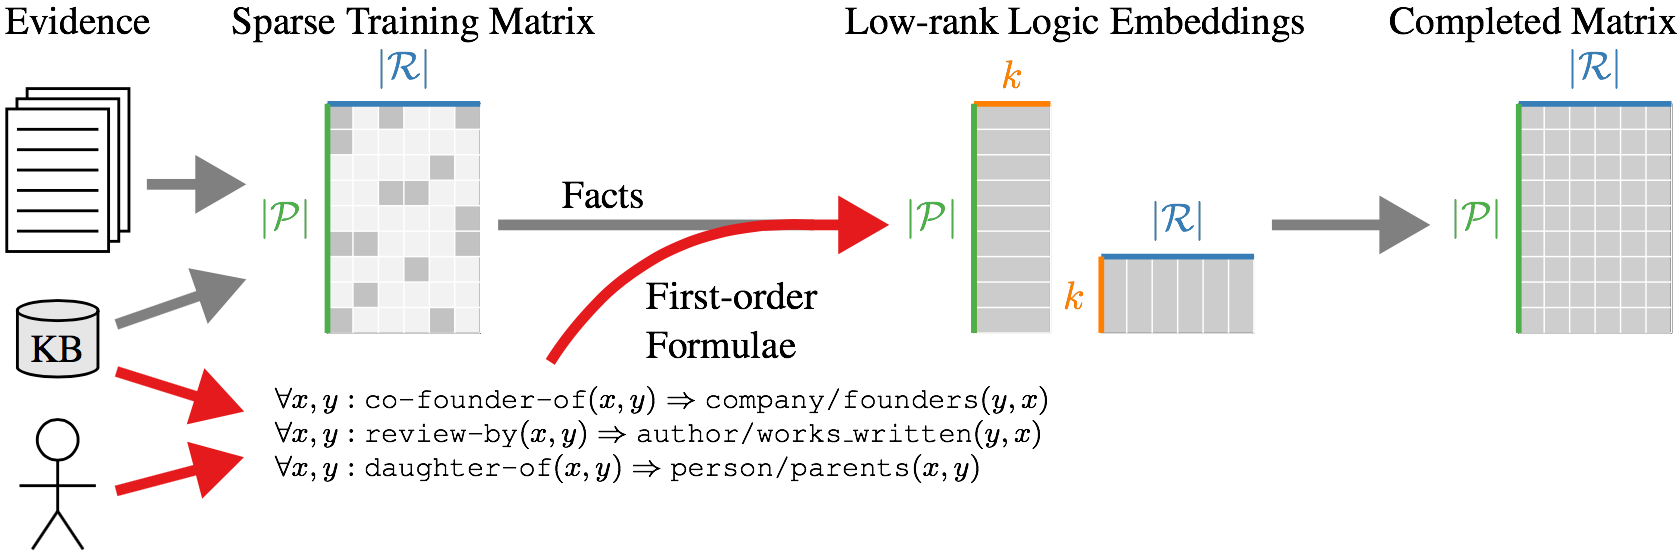
\includegraphics[width=0.9\hsize]{file/overview.png}
  \begin{columns}[c]
   \column{.2\hsize}
   \column{.6\hsize}
  \begin{block}{}
    \centering
  原始矩阵 $|\mathcal{P}|\times|\mathcal{R}|$ \\
  
\resizebox{6cm}{!}{
\begin{tabular}{l|l|l|l|l|l|l|l|l|l|}
\multicolumn{1}{c}{ } & \multicolumn{1}{c}{fr1}  & \multicolumn{1}{c}{fr2}  & \multicolumn{1}{c}{fr3}  & \multicolumn{1}{c}{p1}  & \multicolumn{1}{c}{p2}  & \multicolumn{1}{c}{p3}  & \multicolumn{1}{c}{p4}  & \multicolumn{1}{c}{p5}  & \multicolumn{1}{c}{p6} \tabularnewline \hhline{~|*{9}{-}}
\rowcolor[HTML]{C0C0C0} 
(e1,e2)  & \cellcolor[HTML]{EFEFEF}1 & \cellcolor[HTML]{EFEFEF}0 & \cellcolor[HTML]{EFEFEF}0                      & 0  & 1  & 0  & 0  & 1  & 0  \tabularnewline \hhline{~|*{9}{-}}
\rowcolor[HTML]{C0C0C0} 
(e2,e3)  & \cellcolor[HTML]{EFEFEF}0 & \cellcolor[HTML]{EFEFEF}1 & \cellcolor[HTML]{EFEFEF}0                      & 1  & 0  & 0  & 1  & 0  & 0  \tabularnewline \hhline{~|*{9}{-}}
\rowcolor[HTML]{C0C0C0} 
(e1,e3)  & \cellcolor[HTML]{EFEFEF}0 & \cellcolor[HTML]{EFEFEF}0 & \cellcolor[HTML]{EFEFEF}1                      & 0  & 0  & 1  & 0  & 0  & 0  \tabularnewline \hhline{~|*{9}{-}}
\rowcolor[HTML]{C0C0C0} 
(e1,e10) & \cellcolor[HTML]{EFEFEF}1 & \cellcolor[HTML]{EFEFEF}0 & \cellcolor[HTML]{EFEFEF}0                      & 1  & 0  & 0  & 0  & 0  & 0  \tabularnewline \hhline{~|*{9}{-}}
(e1,e6)  & \cellcolor[HTML]{FFCCC9}1 & \cellcolor[HTML]{FFCCC9}1 & \cellcolor[HTML]{FFCCC9}0                      & 1  & 0  & 0  & 1  & 1  & 0  \tabularnewline \hhline{~|*{9}{-}}
(e1,e8)  & \cellcolor[HTML]{FFCCC9}1 & \cellcolor[HTML]{FFCCC9}0 & \cellcolor[HTML]{FFCCC9}0                      & 1  & 0  & 0  & 0  & 0  & 0  \tabularnewline \hhline{~|*{9}{-}} 
(e3,e7)  & \cellcolor[HTML]{FFCCC9}0 & \cellcolor[HTML]{FFCCC9}1 & \cellcolor[HTML]{FFCCC9}0 & 1  & 0  & 0  & 1  & 0  & 0  \tabularnewline \hhline{~|*{9}{-}}
\end{tabular}
}
  \end{block}
   \column{.2\hsize}
  \end{columns}



}

\frame{
  \frametitle{summary Experiemnt}
  实验框架
  \begin{columns}[c]
   \column{.57\hsize}
   \noindent\scalebox{0.9}{
\begin{tikzpicture}
\tikzstyle{Node}=[draw, rectangle, rounded corners, align=center]
\node [Node, text width=3cm] (rule) {由训练集(\textbf{原始的矩阵})提取\emph{规则集合$\mathfrak{F}$}} ;
\node [Node, text width=2.5cm, right=of rule] (objective) {目标函数$\displaystyle\min_V \sum_{\mathcal{F}\in\mathfrak{F}}\mathcal{L}([\mathcal{F}])$} ;
\node [Node, text width=2.8cm, below=of rule] (MF) {利用\textbf{过滤后的矩阵},分解得到初始实体对向量$v_{(e_i,e_j)}$,关系向量$v_{r_m}$} ;
\node [Node, text width=2.5cm, right=of MF, xshift=1cm] (SGD) {随机梯度下降解得实体对向量$v_{(e_i,e_j)}$,关系向量$v_{r_m}$} ;

\path[-Stealth, blue, thick] 
  (rule) edge [bend left=10] (objective) 
  (rule.south) edge [bend left=30] (MF.north) 
  (MF.east) edge [bend left=10] (SGD.west)
  (objective.south) edge [bend left=30] (SGD.north) 
 ;
\end{tikzpicture}
}

  \column{.4\hsize}
  \begin{itemize}
   \item 不同实验共享相同规则集$\mathfrak{F}$;不同实验“过滤后的矩阵”不同
   \item 一般矩阵分解目标函数$\displaystyle\min_V \sum_{((i, j)}|M(i,j))-v_i\cdot v_j|^2$
   \item 得到最终的向量空间后,判断$(e_i,e_j)$是否含有$r_t$关系,只要判断$\sigma(\mathbf{v_{r_m}}\cdot \mathbf{v_{(e_i, e_j)}})$是否大于阈值
  \end{itemize}

  \end{columns}

}

\frame{
  \begin{itemize}
   \item 矩阵分解(MF) vs 规则抽取(Rule-based)
      \begin{itemize}
       \item MF: 开放域、不需要标注数据(弱监督);完全依赖于KB的质量
	  \begin{itemize}
	   \item 关系出现次数多,预测才好;不出现的无法预测;
	  \end{itemize}

       \item Rule-based: 可以发现新的实体,新的关系;噪声大
      \end{itemize}
   \item 本文动机
      \begin{itemize}
       \item 矩阵分解 和 规则(一阶逻辑(FOL)) 混合
      \end{itemize}
   \item 本文的贡献
      \begin{enumerate}
       \item 如何在矩阵分解前、后利用谓词逻辑
       \item 利用一阶谓词逻辑训练更好的实体对向量、谓词向量
       \item 结合MF,FOL来预测实体的关系
      \end{enumerate}

  \end{itemize}

}

\frame{
  \frametitle{ Notation }
  $\mathcal{P}\subseteq\varepsilon\times\varepsilon$ :实体对$(e_i,e_j)$集合 \\
  $\mathcal{R}$ :关系$fr_i,p_j$集合 \\
  $V$:向量空间$\{v_{fr_1}=\mathbf{v_{r_m}},v_{fr_2},...,v_{p_1}=\mathbf{v_{(e_i,e_j)}},v_{p_2},...\}$ \\
  $\pi_{m}^{e_i,e_j}=\sigma(\mathbf{v_{r_m}},\mathbf{v_{(e_i,e_j)}})$ :实体对与关系的相似性 $\sigma$:sigmoid func
  \begin{itemize}
   \item 一阶谓词
      \begin{itemize}
	\item 原子问题(ground Atom):$professorAt(x,y)$
	\item 复合问题(logical background knowledge):$professorAt(x,y)\Rightarrow emplyeeAt(x,y)$
      \end{itemize}
  \end{itemize}
   评价一阶谓词集合$\mathbf{w}$的好坏 
   \begin{block}{}
    $$p(\mathbf{w}|{V})=\prod_{r_m(e_i,e_j)\in w}\pi_{m}^{e_i,e_j}\prod_{r_m(e_i,e_j)\notin w}(1-\pi_{m}^{e_i,e_j})$$
   \end{block}

}

\frame{
  \frametitle{ Method }
  \begin{enumerate}
   \item 传统方法
      \begin{itemize}
       \item 直接矩阵分解(MF)
       \item 只利用逻辑规则(Inf)
      \end{itemize}
   \item FOL,MF “混合”模型
      \begin{enumerate}
	\item FOL作为预处理 (Pre-Factorization Inference)
	  \begin{itemize}
	  \item 先用FOL改变原始矩阵 $M_{|\mathcal{P}|\times|\mathcal{R}|}$ ,再进行普通矩阵分解
	  \end{itemize}
       \item 将抽取的规则(一阶谓词子集)加入目标函数(Joint Optimization)
       \item 传统矩阵分解生成向量空间$V$,然后使用收集的逻辑规则预测(Post-Factorization Inference)
	  \begin{itemize}
	   \item $\mathcal{F}:(r_s(e_i,e_j) \Rightarrow r_t(e_i,e_j)) \in \mathfrak{F}$:若满足$r_s(e_i,e_j)$, 则预测$r_t(e_i,e_j)$为真
	  \end{itemize}

      \end{enumerate}

  \end{enumerate}

}

\frame{
  \frametitle{一阶逻辑(FOL)注入}
  两种途径\\
      \begin{enumerate}
	\item FOL作为预处理 (Pre-Factorization Inference)
	  \begin{itemize}
	  \item 先用FOL改变原始矩阵 $M_{|\mathcal{P}|\times|\mathcal{R}|}$ ,再进行普通矩阵分解
	  \end{itemize}
       \item 一阶谓词子集加入目标函数(Joint Optimization)
      \end{enumerate}
  
}


\frame{
  \begin{columns}[c]
   \column{.2\hsize}
   \column{.6\hsize}
   \begin{block}{}
    \centering \Large Pre-Factorization Inference\\ (FOL作为预处理)
   \end{block}

   \column{.2\hsize}
  \end{columns}

}

\frame{
  \frametitle{Pre-Factorization Inference(FOL作为预处理)}
  核心:弥补矩阵的稀疏性,增加收集的\emph{一阶逻辑规则$\mathfrak{F}$}与freebase relation之间的关联 \\
  方法:根据逻辑规则,增加原始矩阵 $M_{|\mathcal{P}|\times|\mathcal{R}|}$中值为1的元素个数
  \begin{block}{steps}
   \begin{enumerate}
    \item 收集一阶谓词规则$\mathfrak{F}$
    \item 对$\mathfrak{F}$中每一条规则,比如$\mathbf{F}=\forall x,y:r_s(x,y) \Rightarrow r_t(x,y)$
	\begin{itemize}
	 \item 如果矩阵 $M[(x,y),r_s]$上的值为1,则把$[(x,y),r_t]$上的值置为1
	 \item 递归做下去,直到没有新的1出现
	\end{itemize}
    \item 对更新后的矩阵$M_{|\mathcal{P}|\times|\mathcal{R}|}'$进行传统矩阵分解
    \item 利用$\sigma(\mathbf{v_{r_m}}\cdot \mathbf{v_{(e_i, e_j)}})$预测$(v_{r_m},v_{(e_i, e_j)})$是否应该出现
   \end{enumerate}

  \end{block}

}


\frame{
  \begin{columns}[c]
   \column{.2\hsize}
   \column{.6\hsize}
   \begin{block}{}
    \centering \Large Joint Optimization(组合模型)
   \end{block}

   \column{.2\hsize}
  \end{columns}

}

\frame{
  \frametitle{Joint Optimization(组合模型)}
  核心:把收集的\emph{一阶逻辑规则$\mathfrak{F}$}加入到矩阵分解的目标函数中,训练出更好的属性(关系)向量$v_{r_m}$、实体对向量$v_{(e_i,e_j)}$\\
  训练集的目标函数:$$\displaystyle\min_V \sum_{\mathcal{F}\in\mathfrak{F}}\mathcal{L}([\mathcal{F}])$$
  \begin{block}{}
  \small $[\mathcal{F}]$ is the marginal probability $p(w|V)$ that the formula F is true under the model
  \end{block}
  $\mathcal{L}([\mathcal{F}]):=-\log([\mathcal{F}])$\\
  $V$:向量空间$\{v_{fr_1}=\mathbf{v_{r_m}},v_{fr_2},...,v_{p_1}=\mathbf{v_{(e_i,e_j)}},v_{p_2},...\}$ \\
  $p(\mathbf{w}|{V})=\prod_{r_m(e_i,e_j)\in w}\pi_{m}^{e_i,e_j}\prod_{r_m(e_i,e_j)\notin w}(1-\pi_{m}^{e_i,e_j})$
  
}


\frame{
  \frametitle{边缘分布(marginal probability)}
  \begin{block}{definition}
   对多变量的分布函数,针对某个变量进行求和\emph{(枚举其他变量的所有情况)},所得到的概率分布
  \end{block}
  
  \begin{block}{example}
   联合概率$P(A,B)$,对A的边缘分布为$P_1(A)=\sum_{b\in B}P(A,b)$,对B的边缘分布为$P_2(B)=\sum_{a\in A}P(a,B)$
  \end{block}
  

}

\frame{
  \frametitle{边缘分布(marginal probability)}
  \begin{block}{}
   $p(\mathbf{w}|{V})=\prod_{r_m(e_i,e_j)\in w}\pi_{m}^{e_i,e_j}\prod_{r_m(e_i,e_j)\notin w}(1-\pi_{m}^{e_i,e_j})$\\
  $p(\mathbf{w}|{V})=\prod f_{r_m(e_i,e_j)}=f_{r_m(e_i,e_j)}\times f_{r_n(e_k,e_l)}\times ...$ (相互独立)\\
   \begin{tiny}
   \begin{equation}
    f_{r_m(e_i,e_j)}=
   \begin{cases}
   \pi_{m}^{e_i,e_j} &\mbox{if $r_m(e_i,e_j)\in w$ }\\
   1-\pi_{m}^{e_i,e_j} &\mbox{if $r_m(e_i,e_j)\notin w$ }\\
   \end{cases}
  \end{equation}
  \end{tiny}
  \end{block}
 
 \begin{itemize}
  \item 当$\mathcal{F}$是原子命题时 $[\mathcal{F}]=\pi_{m}^{e_i,e_j}$\\
  \item 当$\mathcal{F}=\mathcal{A}\wedge\mathcal{B}$, $\mathcal{A}$和$\mathcal{B}$是原子命题时, $[\mathcal{F}]=\pi_{m}^{e_i,e_j}\times\pi_{n}^{e_k,e_l}=[\mathcal{A}][\mathcal{B}]$\\
  \item 当$\mathcal{F}=\neg\mathcal{A}$,$\mathcal{A}$是原子命题时,$[\mathcal{F}]=1-[\mathcal{A}]$
 \end{itemize}

  \begin{block}{$\forall[\mathcal{F}]$}
  $\mathcal{F}=\mathcal{A}\vee\mathcal{B}=1-(\neg\mathcal{A})\wedge(\neg\mathcal{B})$\\
  $[\mathcal{A}\vee\mathcal{B}]=[\mathcal{A}]+[\mathcal{B}]-[\mathcal{A}][\mathcal{B}]$\\
  $[\mathcal{A}\Rightarrow\mathcal{B}]=[\mathcal{A}]([\mathcal{B}]-1)+1$...\\
  
  \end{block}

}

\frame{
  \frametitle{Joint Optimization(组合模型)}
  目标函数:$$\displaystyle\min_V \sum_{\mathcal{F}\in\mathfrak{F}}\mathcal{L}([\mathcal{F}])$$
  使用随机梯度下降(stochastic gradient descent)求解
  \begin{block}{}
   \begin{itemize}
    \item $\mathcal{L}([\mathcal{F}]):=-\log([\mathcal{F}])$
    \item 对任意一个$\mathcal{F}$,其只和实体对向量、谓词向量有关
    \item 对任意$\mathcal{L}([\mathcal{F}])$只要求$\partial \mathcal{L}([\mathcal{F}])/\partial v_{r_m}$和$\partial\mathcal{L}([\mathcal{F}])/\partial v_{(e_i,e_j)}$
   \end{itemize}

  \end{block}

}

\frame{
  \frametitle{Joint Optimization(组合模型)}
  $\pi_{m}^{e_i,e_j}=\sigma(\mathbf{v_{r_m}},\mathbf{v_{(e_i,e_j)}})$ \\
  $\mathcal{L}([\mathcal{F}]):=-\log([\mathcal{F}])$
  \begin{columns}[c]
   \column{.55\hsize}
    \begin{block}{$\mathcal{F}= \pi_{m}^{e_i,e_j}$ is a ground atom}
   $\partial [\mathcal{F}]/\partial v_{r_m}=[\mathcal{F}](1-[\mathcal{F}])v_{(e_i,e_j)}$ \\
   $\partial [\mathcal{F}]/\partial v_{(e_i,e_j)}=[\mathcal{F}](1-[\mathcal{F}])v_{r_m}$ \\
   $\partial \mathcal{L}([\mathcal{F}])/\partial v_{r_m}=-[\mathcal{F}]^{-1}\partial [\mathcal{F}]/\partial v_{r_m}$ \\
   $\partial \mathcal{L}([\mathcal{F}])/\partial v_{(e_i,e_j)}=-[\mathcal{F}]^{-1}\partial [\mathcal{F}]/\partial v_{(e_i,e_j)}$
  \end{block}
  
  \column{.4\hsize}
   \begin{block}{$\mathcal{F}$ is a First-order Logic}
   e.g. $\mathcal{F}= \forall x,y:r_s(x,y) \Rightarrow t(x,y)$ \\
   $[\mathcal{F}]=\displaystyle\prod_{(e_i,e_j)\in\mathcal{P}}[\mathcal{F}_{ij}]$ \\
   $\mathcal{L}([\mathcal{F}])=\sum_{(e_i,e_j)\in\mathcal{P}}\mathcal{L}([\mathcal{F}_{ij}])$
  \end{block}
  \end{columns}
  
  \vspace{5mm}
  目标函数:$$\displaystyle\min_V \sum_{\mathcal{F}\in\mathfrak{F}}\mathcal{L}([\mathcal{F}])$$
}

\frame{
  \frametitle{Formulae Extraction and Annotation(一阶逻辑规则$\mathfrak{F}$抽取)}
  
  \begin{enumerate}
   \item 由分解原始矩阵 $M_{|\mathcal{P}|\times|\mathcal{R}|}$ 得到实体对向量、关系向量
   \item 对所有关系对:$(r_s,r_t), r_t\in freebase$
      \begin{enumerate}
       \item 对训练集中的所有实体对$(e_i,e_j)$,计算$[r_s(e_i,e_j) \Rightarrow r_t(e_i,e_j)]$
      \end{enumerate}
   \item 取值最高的100个作为抽取的一阶逻辑规则集合$\mathfrak{F}$
      \begin{itemize}
       \item 其中前36个比较好
      \end{itemize}

  \end{enumerate}
  
  \begin{block}{Formula}
   \begin{small}
    0.97 $\forall x,y: \#2-unit-of-\#1(x, y) \Rightarrow org/parent/child(x, y)$\\
    0.97 $\forall x,y: \#2-city-of-\#1(x, y) \Rightarrow location/containedby(x, y)$\\
    0.97 $\forall x,y: \#2-minister-\#1(x, y) \Rightarrow person/nationality(x, y)$\\
    0.96 $\forall x,y: \#2-minister-\#1(x, y) \Rightarrow person/nationality(x, y)$
   \end{small}
  \end{block}

}

\frame{
  \begin{columns}[c]
   \column{.25\hsize}
   \column{.5\hsize}
   \begin{block}{}
    \centering \Large Experiment
   \end{block}

   \column{.25\hsize}
  \end{columns}

}

\frame{
  \frametitle{Experiment}
  \begin{columns}[c]
   
\column{.5\hsize}
\begin{small}
 
  \begin{block}{1. Zero-shot Relation Learning}
   \begin{itemize}
    \item 舍去所有freebase relation信息,\emph{训练数据中freebase relation的列都置为0}(模拟新关系的发现)
   \end{itemize}

  \end{block}

  \begin{block}{2. Relations with Few Distant Labels}
      \begin{itemize}
        \item 给出部分freebase relation信息. 给出率为0时退化为实验1
      \end{itemize}

  \end{block}

  \begin{block}{3. Comparison on Complete Data}
      \begin{itemize}
       \item 给出全部freebase relation信息. 等价于实验2中给出率为100\%
      \end{itemize}

  \end{block}
\end{small}

  
\column{.47\hsize}

  原始矩阵 $|\mathcal{P}|\times|\mathcal{R}|$ \\
\resizebox{6cm}{!}{
\begin{tabular}{l|l|l|l|l|l|l|l|}
\multicolumn{1}{c}{} & \multicolumn{1}{c}{fr1}  & \multicolumn{1}{c}{fr2}  & \multicolumn{1}{c}{fr3}  & \multicolumn{1}{c}{p1}  & \multicolumn{1}{c}{p2}  \tabularnewline \hhline{~|*{5}{-}}
\rowcolor[HTML]{C0C0C0} 
(e1,e2)  & \cellcolor[HTML]{EFEFEF}1 & \cellcolor[HTML]{EFEFEF}0 & \cellcolor[HTML]{EFEFEF}0                      & 0  & 1  \tabularnewline \hhline{~|*{5}{-}}
\rowcolor[HTML]{C0C0C0} 
(e2,e3)  & \cellcolor[HTML]{EFEFEF}0 & \cellcolor[HTML]{EFEFEF}1 & \cellcolor[HTML]{EFEFEF}0                      & 1  & 0   \tabularnewline \hhline{~|*{5}{-}}
\rowcolor[HTML]{C0C0C0} 
(e1,e3)  & \cellcolor[HTML]{EFEFEF}0 & \cellcolor[HTML]{EFEFEF}0 & \cellcolor[HTML]{EFEFEF}1                      & 0  & 0   \tabularnewline \hhline{~|*{5}{-}}
\rowcolor[HTML]{C0C0C0} 
(e1,e10) & \cellcolor[HTML]{EFEFEF}1 & \cellcolor[HTML]{EFEFEF}0 & \cellcolor[HTML]{EFEFEF}0                      & 1  & 0   \tabularnewline \hhline{~|*{5}{-}}
(e1,e6)  & \cellcolor[HTML]{FFCCC9}1 & \cellcolor[HTML]{FFCCC9}1 & \cellcolor[HTML]{FFCCC9}0                      & 1  & 0   \tabularnewline \hhline{~|*{5}{-}}
(e1,e8)  & \cellcolor[HTML]{FFCCC9}1 & \cellcolor[HTML]{FFCCC9}0 & \cellcolor[HTML]{FFCCC9}0                      & 1  & 0   \tabularnewline \hhline{~|*{5}{-}} 
(e3,e7)  & \cellcolor[HTML]{FFCCC9}0 & \cellcolor[HTML]{FFCCC9}1 & \cellcolor[HTML]{FFCCC9}0 & 1  & 0   \tabularnewline \hhline{~|*{5}{-}}
\end{tabular}
}

  \end{columns}


}

\frame{
  \frametitle{Experiemnt}
  \begin{columns}[c]
   \column{.57\hsize}
   以 Joint Optimization为例\\
  \vspace{5mm}
   \noindent\scalebox{0.9}{
\begin{tikzpicture}
\tikzstyle{Node}=[draw, rectangle, rounded corners, align=center]
\node [Node, text width=3cm] (rule) {由训练集(\textbf{原始的矩阵})提取\emph{规则集合$\mathfrak{F}$}} ;
\node [Node, text width=2.5cm, right=of rule] (objective) {目标函数$\displaystyle\min_V \sum_{\mathcal{F}\in\mathfrak{F}}\mathcal{L}([\mathcal{F}])$} ;
\node [Node, text width=2.8cm, below=of rule] (MF) {利用\textbf{过滤后的矩阵},分解得到初始实体对向量$v_{(e_i,e_j)}$,关系向量$v_{r_m}$} ;
\node [Node, text width=2.5cm, right=of MF, xshift=1cm] (SGD) {随机梯度下降解得实体对向量$v_{(e_i,e_j)}$,关系向量$v_{r_m}$} ;

\path[-Stealth, blue, thick] 
  (rule) edge [bend left=10] (objective) 
  (rule.south) edge [bend left=30] (MF.north) 
  (MF.east) edge [bend left=10] (SGD.west)
  (objective.south) edge [bend left=30] (SGD.north) 
 ;
\end{tikzpicture}
}

  \column{.4\hsize}
  \begin{itemize}
   \item 不同实验共享相同规则集$\mathfrak{F}$
   \item 不同实验“过滤后的矩阵”不同
   \item 一般矩阵分解目标函数$\displaystyle\min_V \sum_{((i, j)}|M(i,j))-v_i\cdot v_j|^2$
   \item 得到最终的向量空间后,判断$(e_i,e_j)$是否含有$r_t$关系,只要判断$\sigma(\mathbf{v_{r_m}},\mathbf{v_{(e_i,e_j)}})$是否大于阈值
  \end{itemize}

  \end{columns}

}

\frame{
  \frametitle{dataset}
  \begin{block}{}
   $M_{|\mathcal{P}|\times|\mathcal{R}|}$: 41913 entity-pairs × 4111 relations(151 freebase relation)\\ 
   118781 training facts(7293 belong to freebase) \\
  \end{block}
  结果使用MAP和wMAP评价
  \begin{block}{weighted Mean Avarage Precision(wMAP)}
   average precision for each relation is weighted by the relation’s number of true facts
  \end{block}

}

\frame{
  \frametitle{1. Zero-shot Relation Learning}
  \begin{center}
   
  \centering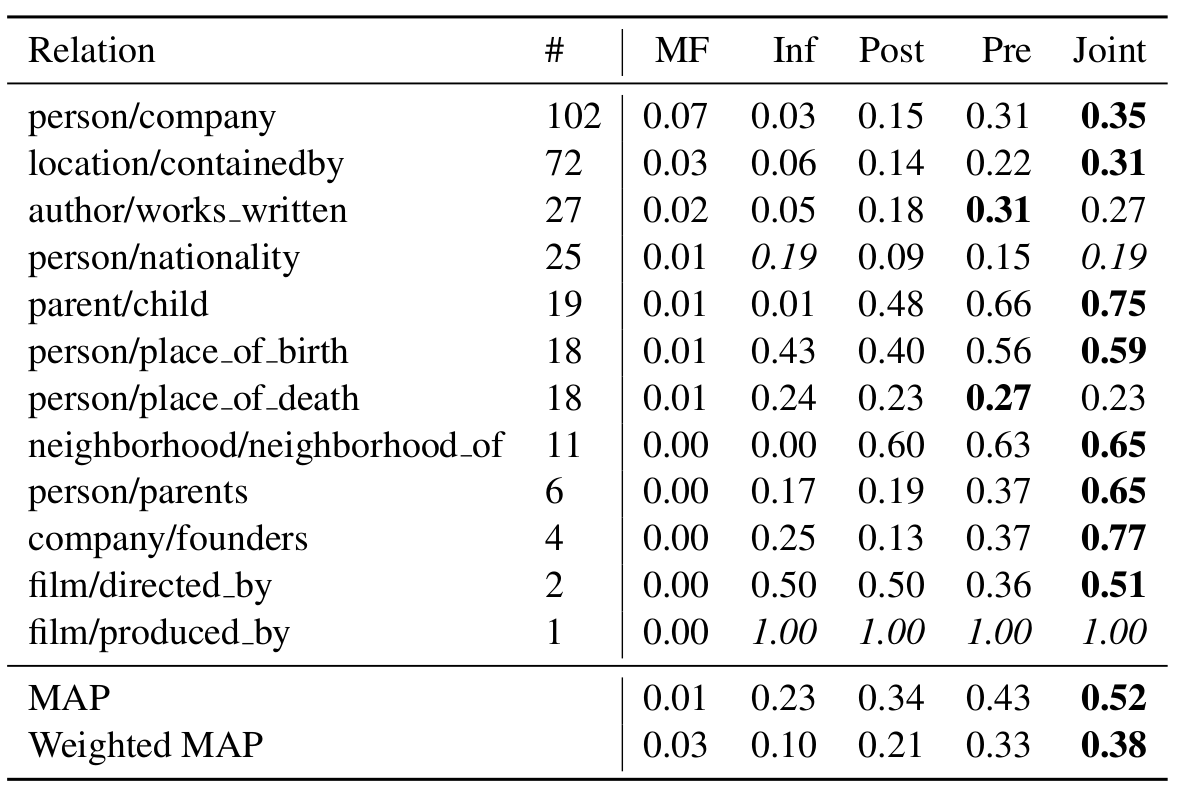
\includegraphics[width=0.7\hsize]{file/test1.png} \\
  \end{center}
  
  MF失败:不能预测未出现过的关系\\
  Inf和Post效果差:两者采用的向量空间太差,没有优化、、
}

\frame{
  \frametitle{experiment 2. 3.}
  左:实验2, 右:实验3\\
  \centering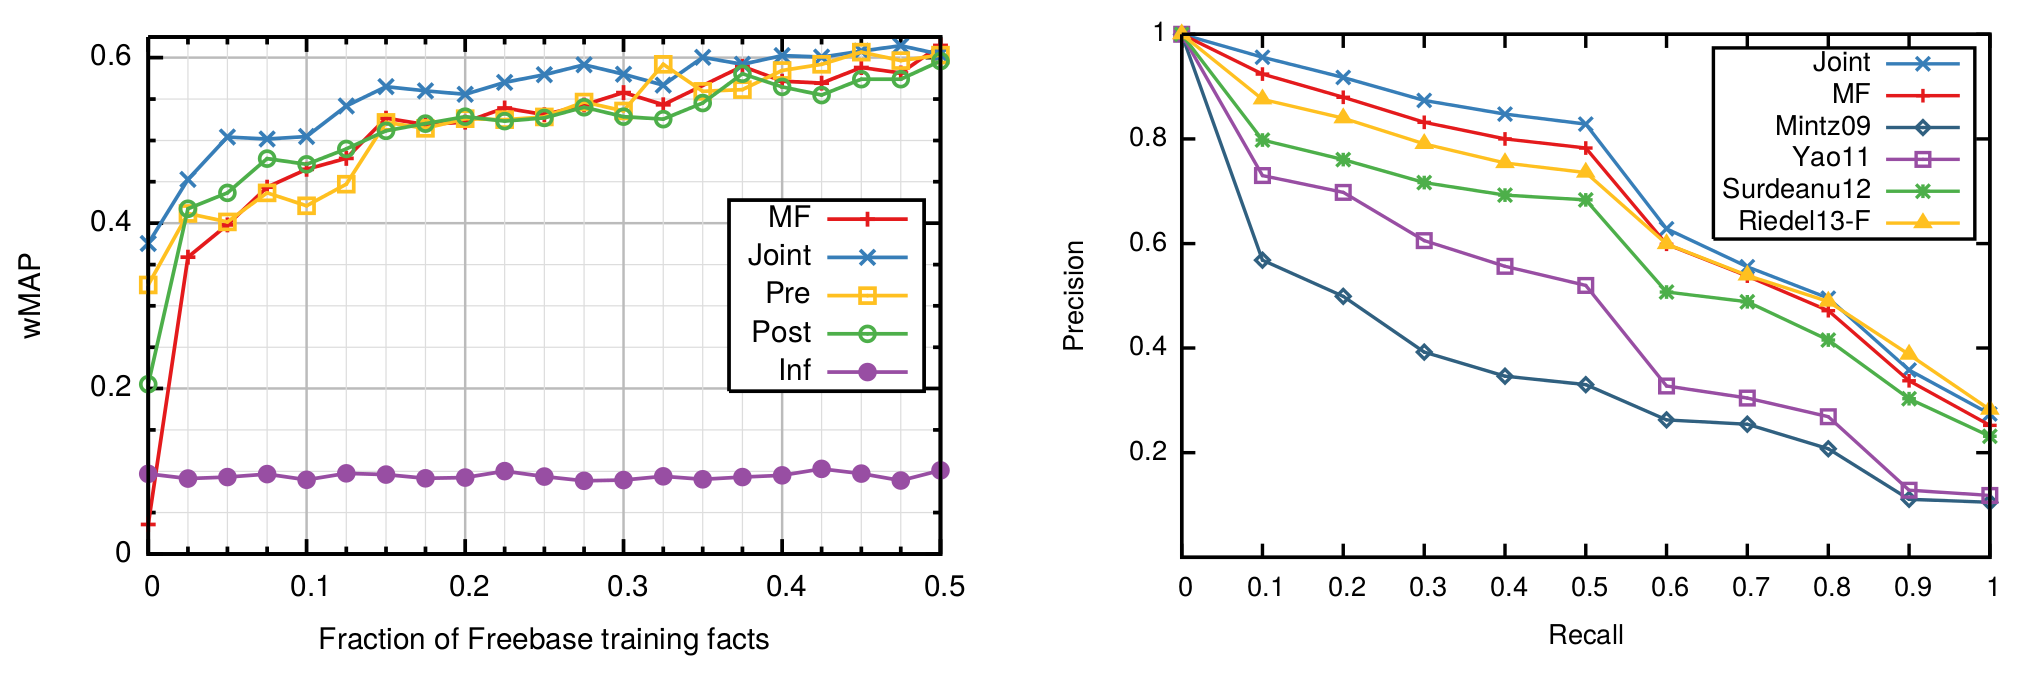
\includegraphics[width=1\hsize]{file/test23.png}\\
  Inf没有考虑freebase relation与pattern“共现”,因而无变化
}

\frame{
  
  \begin{center}
   \Large 谢谢
  \end{center}
}
\frame{
  \frametitle{Append: Mean Avarage Precision(MAP)}
  \centering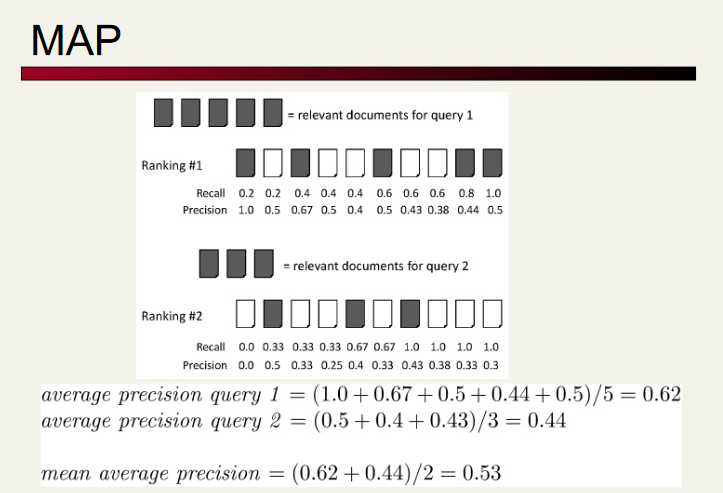
\includegraphics[width=0.9\hsize]{file/244943387_o.png}
}



\end{document}